% $Id: template.tex 11 2007-04-03 22:25:53Z jpeltier $

\documentclass{vgtc}                          % final (conference style)
%\documentclass[review]{vgtc}                 % review
%\documentclass[widereview]{vgtc}             % wide-spaced review
%\documentclass[preprint]{vgtc}               % preprint
%\documentclass[electronic]{vgtc}             % electronic version

%% Uncomment one of the lines above depending on where your paper is
%% in the conference process. ``review'' and ``widereview'' are for review
%% submission, ``preprint'' is for pre-publication, and the final version
%% doesn't use a specific qualifier. Further, ``electronic'' includes
%% hyperreferences for more convenient online viewing.

%% Please use one of the ``review'' options in combination with the
%% assigned online id (see below) ONLY if your paper uses a double blind
%% review process. Some conferences, like IEEE Vis and InfoVis, have NOT
%% in the past.

%% Figures should be in CMYK or Grey scale format, otherwise, colour 
%% shifting may occur during the printing process.

%% These few lines make a distinction between latex and pdflatex calls and they
%% bring in essential packages for graphics and font handling.
%% Note that due to the \DeclareGraphicsExtensions{} call it is no longer necessary
%% to provide the the path and extension of a graphics file:
%% \includegraphics{diamondrule} is completely sufficient.
%%
\ifpdf%                                % if we use pdflatex
  \pdfoutput=1\relax                   % create PDFs from pdfLaTeX
  \pdfcompresslevel=9                  % PDF Compression
  \pdfoptionpdfminorversion=7          % create PDF 1.7
  \ExecuteOptions{pdftex}
  \usepackage{graphicx}                % allow us to embed graphics files
  \DeclareGraphicsExtensions{.pdf,.png,.jpg,.jpeg} % for pdflatex we expect .pdf, .png, or .jpg files
\else%                                 % else we use pure latex
  \ExecuteOptions{dvips}
  \usepackage{graphicx}                % allow us to embed graphics files
  \DeclareGraphicsExtensions{.eps}     % for pure latex we expect eps files
\fi%

%% it is recomended to use ``\autoref{sec:bla}'' instead of ``Fig.~\ref{sec:bla}''
\graphicspath{{figures/}{pictures/}{images/}{./}} % where to search for the images

\usepackage{microtype}                 % use micro-typography (slightly more compact, better to read)
\PassOptionsToPackage{warn}{textcomp}  % to address font issues with \textrightarrow
\usepackage{textcomp}                  % use better special symbols
\usepackage{mathptmx}                  % use matching math font
\usepackage{times}                     % we use Times as the main font
\renewcommand*\ttdefault{txtt}         % a nicer typewriter font
\usepackage{cite}                      % needed to automatically sort the references
\usepackage{tabu}                      % only used for the table example
\usepackage{booktabs}                  % only used for the table example
%% We encourage the use of mathptmx for consistent usage of times font
%% throughout the proceedings. However, if you encounter conflicts
%% with other math-related packages, you may want to disable it.

\usepackage{amsmath}


%% If you are submitting a paper to a conference for review with a double
%% blind reviewing process, please replace the value ``0'' below with your
%% OnlineID. Otherwise, you may safely leave it at ``0''.
\onlineid{0}

%% declare the category of your paper, only shown in review mode
\vgtccategory{Research}

%% allow for this line if you want the electronic option to work properly
\vgtcinsertpkg

%% In preprint mode you may define your own headline. If not, the default IEEE copyright message will appear in preprint mode.
%\preprinttext{To appear in an IEEE VGTC sponsored conference.}

%% This adds a link to the version of the paper on IEEEXplore
%% Uncomment this line when you produce a preprint version of the article 
%% after the article receives a DOI for the paper from IEEE
%\ieeedoi{xx.xxxx/TVCG.201x.xxxxxxx}


%% Paper title.

\title{A Plot is Worth a Thousand Tests: Assessing Residual Diagnostics with the Lineup Protocol}

%% This is how authors are specified in the conference style

%% Author and Affiliation (single author).
%%\author{Roy G. Biv\thanks{e-mail: roy.g.biv@aol.com}}
%%\affiliation{\scriptsize Allied Widgets Research}

%% Author and Affiliation (multiple authors with single affiliations).
%%\author{Roy G. Biv\thanks{e-mail: roy.g.biv@aol.com} %
%%\and Ed Grimley\thanks{e-mail:ed.grimley@aol.com} %
%%\and Martha Stewart\thanks{e-mail:martha.stewart@marthastewart.com}}
%%\affiliation{\scriptsize Martha Stewart Enterprises \\ Microsoft Research}

%% Author and Affiliation (multiple authors with multiple affiliations)
\author{Weihao Li\thanks{e-mail: weihao.li@monash.edu}\\ %
        \scriptsize Monash University %
\and Dianne Cook\thanks{e-mail: dicook@monash.edu}\\ %
     \scriptsize Monash University %
\and Emi Tanaka\thanks{e-mail: emi.tanaka@anu.edu.au}\\ %
     \scriptsize Australian National University %
\and Susan VanderPlas\thanks{e-mail: susan.vanderplas@unl.edu}\\ %
     \scriptsize University of Nebraska–Lincoln}

%% A teaser figure can be included as follows
% \teaser{
%   \centering
%   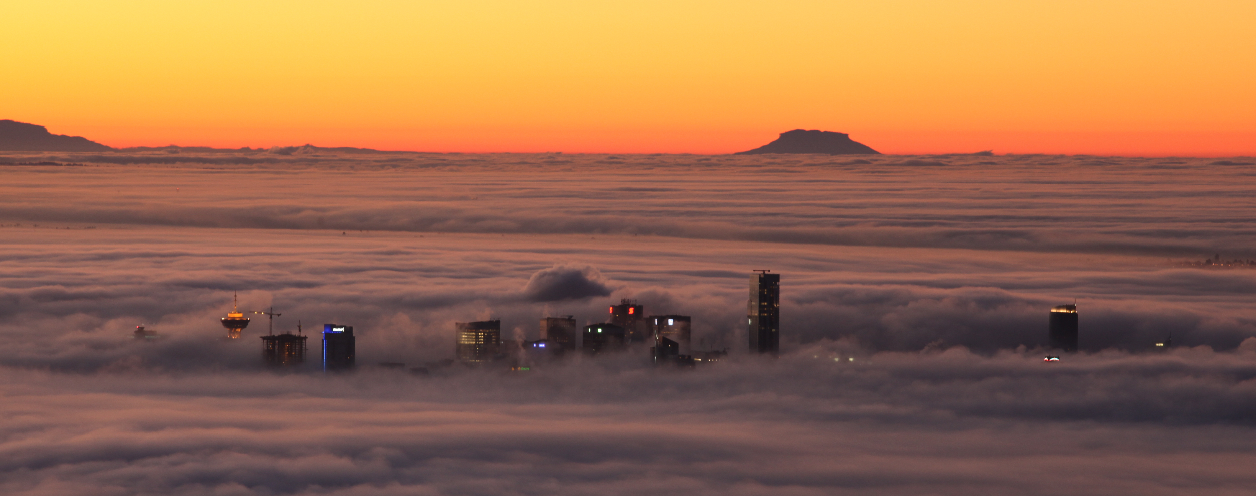
\includegraphics[width=\linewidth]{CypressView}
%   \caption{In the Clouds: Vancouver from Cypress Mountain. Note that the teaser may not be wider than the abstract block.}
%   \label{fig:teaser}
% }

%% Abstract section.
\abstract{Regression experts consistently recommend plotting residuals for model diagnosis, despite the availability of many numerical hypothesis test procedures designed to use residuals to assess problems with a model fit. Here we provide evidence for why this is good advice using data from a visual inference experiment. We show how conventional tests are too sensitive, which means that too often the conclusion would be that the model fit is inadequate. The experiment uses the lineup protocol which puts a residual plot in the context of null plots. This helps generate reliable and consistent reading of residual plots for better model diagnosis. The lineup protocol also detects a range of departures from good residuals simultaneously.%
} % end of abstract

%% ACM Computing Classification System (CCS). 
%% See <http://www.acm.org/about/class> for details.
%% We recommend the 2012 system <http://www.acm.org/about/class/class/2012>
%% For the 2012 system use the ``\CCScatTwelve'' which command takes four arguments.
%% The 1998 system <http://www.acm.org/about/class/class/2012> is still possible
%% For the 1998 system use the ``\CCScat'' which command takes four arguments.
%% In both cases the last two arguments (1998) or last three (2012) can be empty.

\CCScatlist{
  \CCScatTwelve{Mathematics of computing}{Probability and statistics}{Statistical paradigms}{Regression analysis}{};
  \CCScatTwelve{Mathematics of computing}{Probability and statistics}{Statistical paradigms}{Statistical graphics}{}
}

%\CCScatlist{
  %\CCScat{H.5.2}{User Interfaces}{User Interfaces}{Graphical user interfaces (GUI)}{};
  %\CCScat{H.5.m}{Information Interfaces and Presentation}{Miscellaneous}{}{}
%}

%% Copyright space is enabled by default as required by guidelines.
%% It is disabled by the 'review' option or via the following command:
% \nocopyrightspace

%%%%%%%%%%%%%%%%%%%%%%%%%%%%%%%%%%%%%%%%%%%%%%%%%%%%%%%%%%%%%%%%
%%%%%%%%%%%%%%%%%%%%%% START OF THE PAPER %%%%%%%%%%%%%%%%%%%%%%
%%%%%%%%%%%%%%%%%%%%%%%%%%%%%%%%%%%%%%%%%%%%%%%%%%%%%%%%%%%%%%%%%

\begin{document}

%% The ``\maketitle'' command must be the first command after the
%% ``\begin{document}'' command. It prepares and prints the title block.

%% the only exception to this rule is the \firstsection command
\firstsection{Introduction}

\maketitle

%% \section{Introduction} %for journal use above \firstsection{..} instead

In linear regression analysis, studying the residuals from a model fit is a common
diagnostic activity. Residuals summarise what is not captured by the
model, and thus provide the capacity to identify what might be wrong. 
Linear regression is a well-established procedure, and there is
considerable literature describing diagnostic procedures, e.g.
\cite{draper1998applied}, \cite{montgomery1982introduction} and
\cite{cook1982residuals}. Interestingly, despite the abundance of
residual-based conventional tests, ALL of these writings advise that 
plotting residuals is an essential tool for diagnosing regression model 
problems:

\begin{quote}
\emph{Some most useful checks allowed by data plots should be done on a
routine basis for every regression.} \cite{draper1998applied}
\end{quote}

\begin{quote}
\emph{Such formal and informal procedures are complementary, and both
have a place in residual analysis.} \cite{cook1982residuals}
\end{quote}

\begin{quote}
\emph{In our experience, statistical tests on regression model residuals
are not widely used. In most practical situations the residual plots are
more informative than the corresponding tests. However, since residual
plots do require skill and experience to interpret, the statistical
tests may occasionally prove useful.} \cite{montgomery1982introduction}
\end{quote}

\noindent The common wisdom of experts is that plotting the residuals is
indispensable for diagnosing model fits. The ubiquity of this advice is
\emph{curious}.

While examining the scatterplots of residuals, if there are any visually 
discoverable patterns, the model is potentially inadequate or incorrectly 
specified. In general,
one looks for noticeable departures from the model such as non-linear
pattern or heteroskedasticity. However, correctly 
judging whether NO pattern exists in a residual plot is a
difficult task for humans. Humans will almost always see a pattern (see
\cite{kahneman2011thinking}), so the question that really needs
answering is whether any pattern perceived is consistent with
randomness, purely sampling variability, or noise. 

To address the issue of over-interpretation, we can examine the plot in
the context of natural sampling variability assumed by the model, called
the lineup protocol, as proposed in \cite{buja2009statistical}. 
The protocol consists of \(m\) randomly placed plots, where one plot is the
data plot, and the remaining \(m - 1\) plots, referred to as the
\emph{null plots}, are constructed using the same graphical procedure as
the data plot but the data is replaced with null data that is generated
in a manner consistent with the null hypothesis, \(H_0\). 
Computing the \(p\)-value requires that the 
lineup be examined by a number of human judges, 
each asked to select the most different plot. 
A small $p$-value would result from a substantial number 
selecting the data plot. Under \(H_0\), 
it is expected that the data plot would have no distinguishable difference 
from the null plots, and the human judge would only select the data plot 
by chance.
\autoref{fig:first-example-lineup} is an example of a lineup
protocol. If the data plot at position \(2^3 + 1\) is identifiable, then
it is evidence for the rejection of \(H_0\). Otherwise, 
we fail to reject \(H_0\). 


\begin{figure}[tb]
 \centering % avoid the use of \begin{center}...\end{center} and use \centering instead (more compact)
 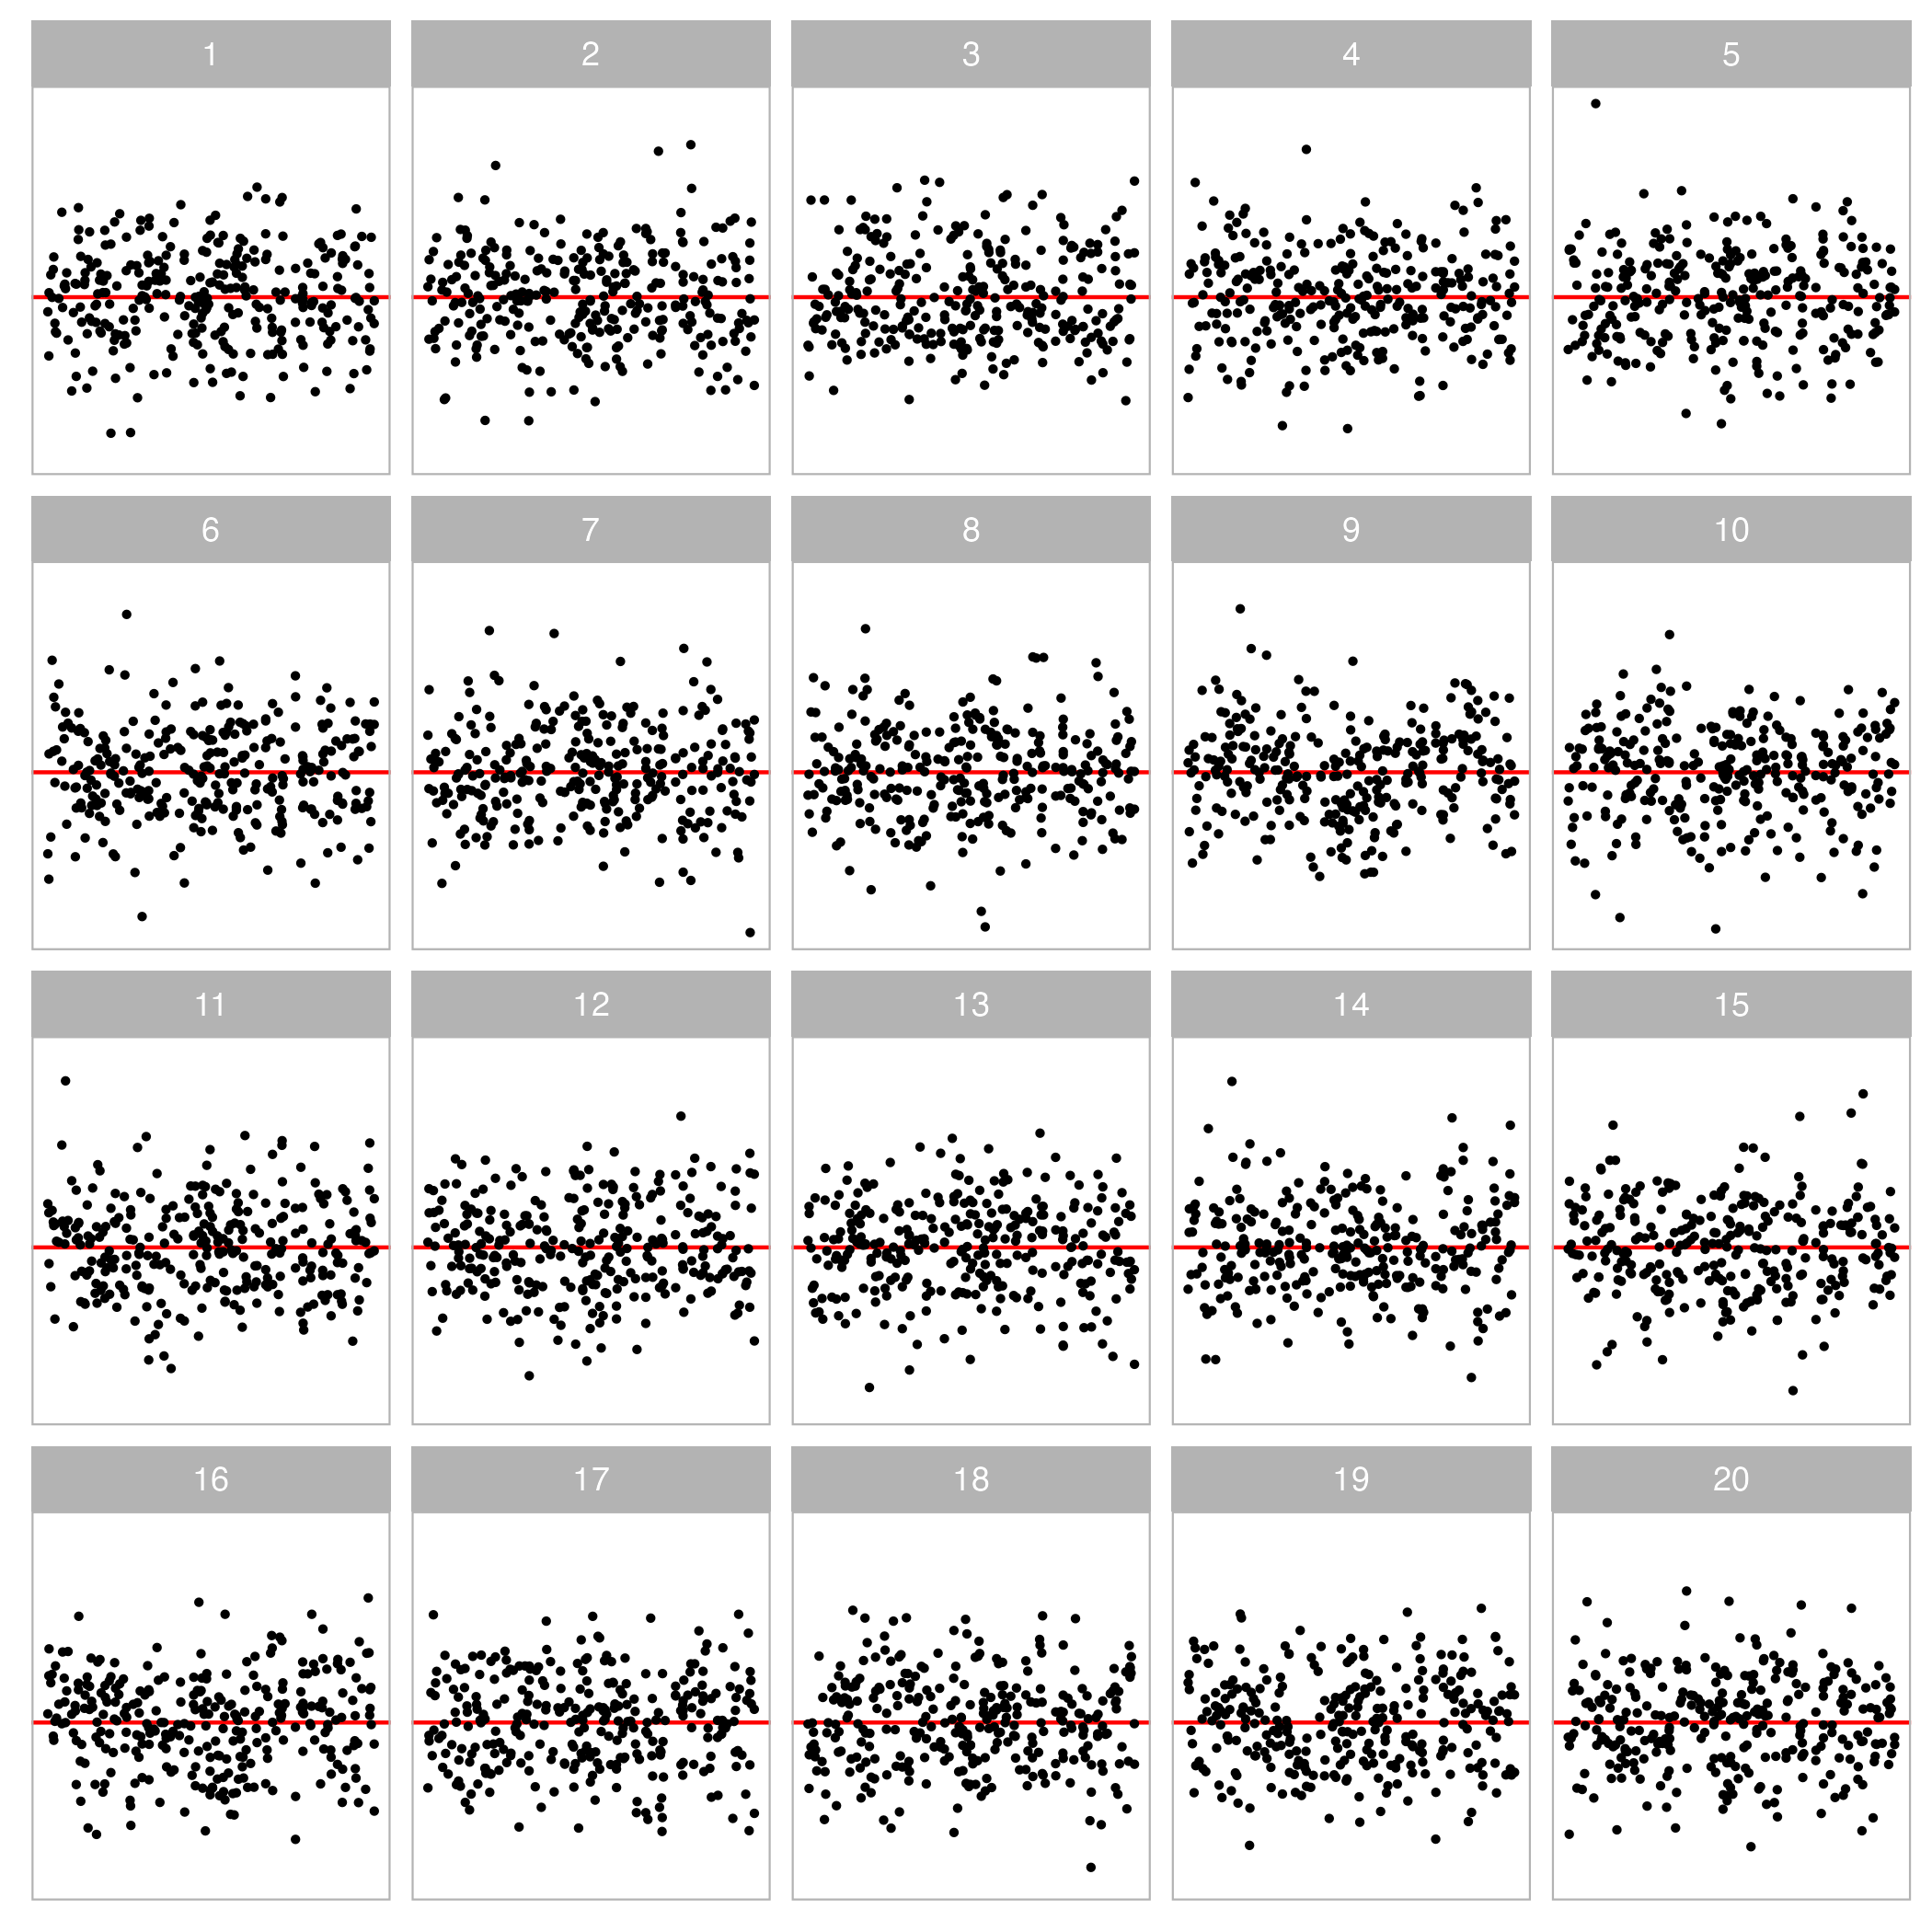
\includegraphics[width=\columnwidth]{131}
 \caption{Visual testing is conducted using a lineup, as in the example here. The residual plot computed from the observed data (plot $2^3 + 1$) is embedded among 19 null plots, where the residuals are simulated from a standard error model.}
 \label{fig:first-example-lineup}
\end{figure}

In this study, we assessed the advice of plotting residuals in regression 
diagnostics by comparing conventional residual-based testing 
and visual testing in a perceptual experiment.

\section{Experimental design}
\label{sec:experimental-design}

Our experiment was conducted over three data collection periods. 
Data collection period I was designed to study the ability of
participants to detect the effect of a non-linear term
\(\boldsymbol{z}\) constructed using Hermite polynomials formulate as \(\boldsymbol{y} = 1 + \boldsymbol{x} + \boldsymbol{z} + \boldsymbol{\varepsilon},~ \boldsymbol{z} \propto He_j(\boldsymbol{x}) ~\text{and}~ \boldsymbol{\varepsilon} \sim N(\boldsymbol{0}, \sigma^2\boldsymbol{I}).\) The null regression model used to fit the realizations generated is formulated as 
\(\boldsymbol{y} = \beta_0 + \beta_1 \boldsymbol{x} + \boldsymbol{u}.\) Since 
\(z = O(x^j)\), for \(j > 1\), \(z\) is a higher order term left
out of the null regression, which will result in model misspecification.

Data collection period II was designed to study the ability of
participants to detect the heteroskedasticity under a simple linear
regression model setting formulated as 
\(\boldsymbol{y} = 1 + \boldsymbol{x} + \boldsymbol{\varepsilon}, ~ \boldsymbol{\varepsilon} \sim N(\boldsymbol{0}, 1 + (2 - |a|)(\boldsymbol{x} - a)^2b \boldsymbol{I}).\)
The same null regression model was used to fit the realizations. 
For \(b \neq 0\), the variance-covariance matrix of the error term
\(\boldsymbol{\varepsilon}\) is correlated with the predictor
\(\boldsymbol{x}\), which will lead to the presence of
heteroskedasticity.

In visual \(p\)-value caculation \cite{vanderplas2021statistical}, 
the parameter \(\alpha\) of the dirichlet distribution usually 
needs to be estimated using data collected from the experiment. 
Thus, we recorded human responses to null lineups in data collection 
period III.

Overall, we
collected 7974 evaluations on 1152 unique lineups performed by 443
participants throughout three data collection periods.

\section{Results}
\label{sec:results}

\begin{figure}[tb]
 \centering % avoid the use of \begin{center}...\end{center} and use \centering instead (more compact)
 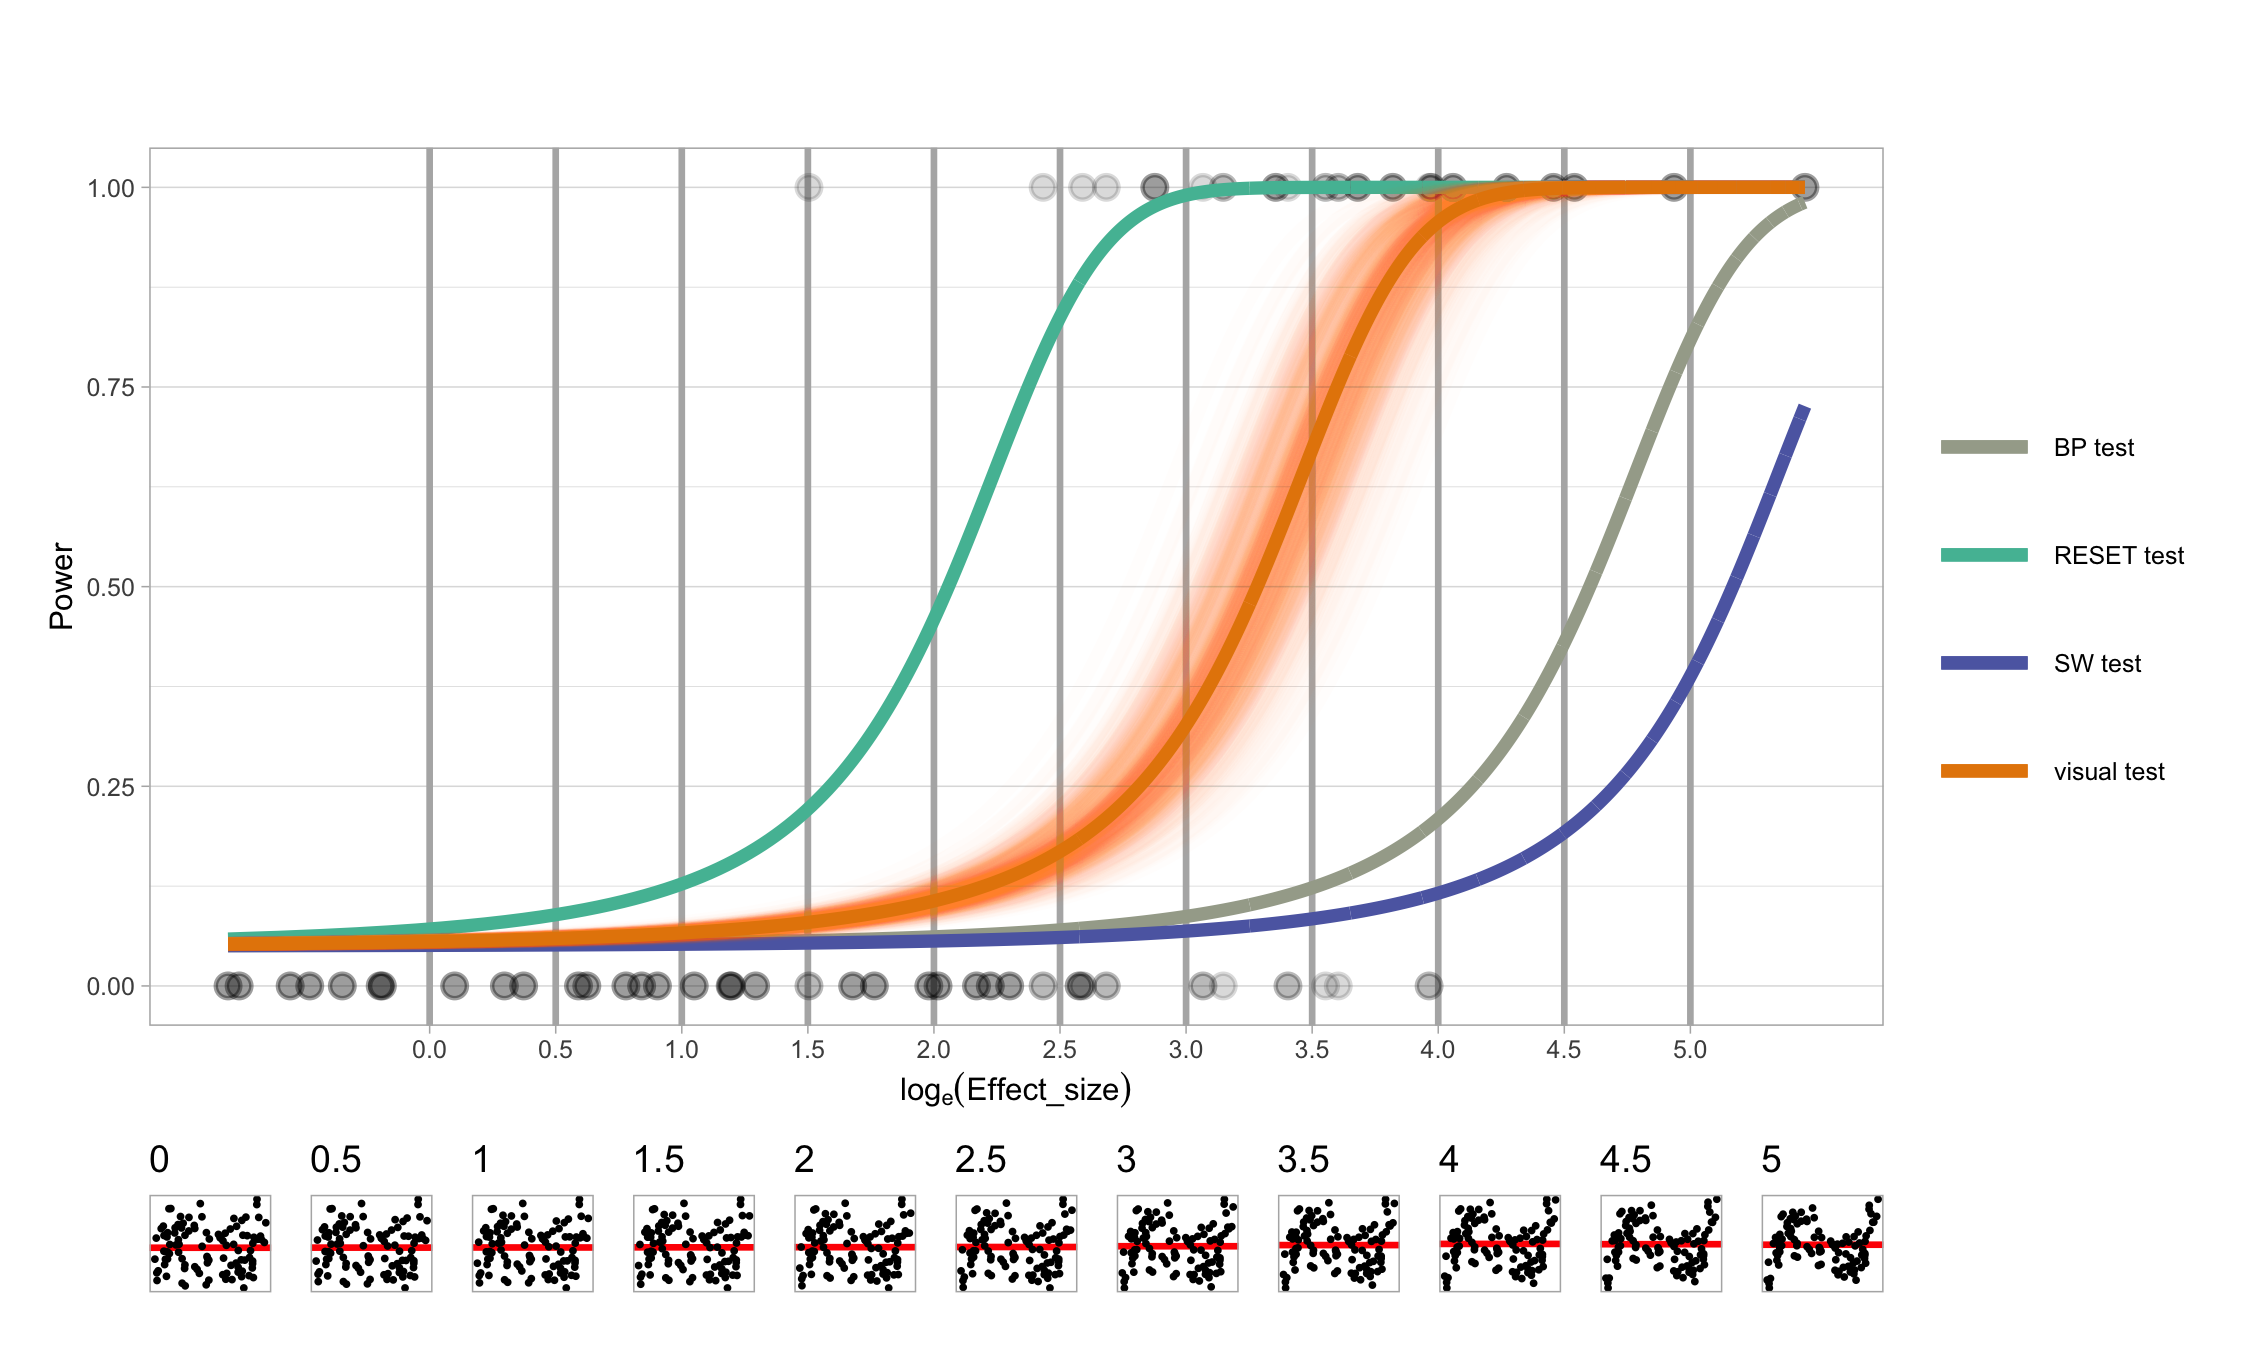
\includegraphics[width=\columnwidth]{polypower-1}
 \caption{Comparison of power between different tests for non-linear patterns. The power curves are estimated using logistic regression, and the horizontal lines of dots represent non-reject and reject results from visual tests for each lineup. The visual test has multiple power curves estimated from bootstrap samples. The row of scatterplots at the bottom are examples of residual plots corresponding to the specific effect sizes marked by vertical lines in the main plot.}
 \label{fig:polypower}
\end{figure}

\autoref{fig:polypower} compares the power for the different tests
for non-linear structure in the residuals, where the effect size is 
quantified via an approach based on Kullback-Leibler divergence, 
coupled with simulation. The test with the uniformly
higher power is the Ramsey Regression Equation
Specification Error Test (RESET) \cite{ramsey1969tests}, 
one that specifically tests for
non-linearity. Note that the Breusch-Pagan (BP) test \cite{breusch1979simple}
and Shapiro-Wilk (SW) normality test \cite{shapiro1965analysis} 
have much lower power,
which is expected because they are not designed to detect non-linearity.
The bootstrapped power curves for the visual test are effectively a
shift right from that of the RESET test. This means that the RESET test
will reject at a lower effect size (less structure) than the visual
test, but otherwise the performance will be similar. In other words, the
RESET test is more sensitive than the visual test. This is not
necessarily a good feature for the purposes of diagnosing model defects:
If we scan the residual plot examples at the bottom, we might argue that
the non-linearity is not sufficiently problematic until an effect size
of around 3 or 3.5. The RESET test would reject closer to an effect size
of 2, but the visual test would reject closer to 3.25, for a significance
level of 0.05. The visual test matches the robustness of the model to
(minor) violations of assumptions much better.

\autoref{fig:first-example-lineup} is an example where the 
RESET test would reject \(H_0\)
(\(p\text{-value} = 2 \times 10^{-9}\)), 
but a visual test would not (visual \(p\text{-value} = 0.530\)), 
when the effect size (\(log_e(\text{Effect}) = 2.68\)) is particularly small. 
Only one out of eleven participants identified the data plot for this lineup. 
It can be also seen from the lineup that there is no
obvious non-linear patterns exhibited in the data plot. 
In this case, we can argue that the fitted model is a good enough 
approximation to the underlying data genearting process.

Similar findings can be extracted for the heteroskedasticity pattern so 
we will not repeat the discussion here.

\section{Conclusion}
\label{sec:conclusion}

Regression analysis experts suggest that residual plots are
indispensable methods for assessing model fit. We conducted a perceptual
experiment using visual inference to assess this oft-repeated advice.
The experiment tested two primary departures from good residuals:
non-linearity and heteroskedasticity.

We found that conventional residual-based statistical tests are more
sensitive to weak departures than visual tests.
Conventional tests often reject
when departures in the form of non-linearity and heteroskedasticity are
not visibly different from null residual plots.

While it might be argued that the conventional tests are correctly
detecting small but real effects, this can also be seen as the
conventional tests are rejecting unnecessarily. Many of these rejections
happen even when downstream analysis and results would not be
significantly affected by the small departures from a good fit. The
results from human evaluations provide a more practical solution, which
reinforces the statements from regression experts that residual plots
are an indispensable method for model diagnostics.

It is important to note that residual plots need to be delivered as a
lineup, embedded in a field of null plots. A residual plot may contain
many visual features, but some are caused by the characteristics of the
predictors and the randomness of the error, not by the violation of the
model assumptions. The lineup enables a careful calibration for
reading structure in residual plots.

%% if specified like this the section will be committed in review mode
% \acknowledgments{
% The authors wish to thank A, B, and C. This work was supported in part by
% a grant from XYZ.}

%\bibliographystyle{abbrv}
\bibliographystyle{abbrv-doi}
%\bibliographystyle{abbrv-doi-narrow}
%\bibliographystyle{abbrv-doi-hyperref}
%\bibliographystyle{abbrv-doi-hyperref-narrow}

\bibliography{template}
\end{document}
